%% Artigo final do Mini-Projeto — Computação Natural (PPGCC/UFMG, 2026/2)
%% Formato ACM exigido pelo enunciado (Fase 4): classe acmart, modelo sigconf (duas colunas).
%% A opção nonacm retira o bloco de direitos autorais, CCS e formato de referência da ACM,
%% que não se aplicam a um trabalho de disciplina.
%%
%% Estrutura: o preâmbulo fica aqui; cada seção em secoes/; tabelas/ e figuras/ são gerados por
%% ../scripts/figuras.py a partir de ../../results/*.json (não editar à mão).
%% Compilar: `make` em report/ (ou `just report` na raiz).

\documentclass[sigconf,nonacm]{acmart}

\usepackage[T1]{fontenc}
\usepackage[utf8]{inputenc}
\usepackage[brazilian]{babel}
\usepackage{enumitem}
\usepackage{tabularx}
\usepackage{tikz}
\usetikzlibrary{positioning}

\setlist{nosep, leftmargin=*}
\graphicspath{{figuras/}}

\newcommand{\PN}{\mathrm{PN}}
\newcommand{\PS}{\mathrm{PS}}
\newcommand{\E}{\mathbb{E}}
%% Corpo de tabela gerado (tabelas/<nome>.tex). Usa a primitiva \@@input, que é expansível:
%% com \input, um \bottomrule logo depois do arquivo dá "Misplaced \noalign".
\makeatletter
\newcommand{\tabela}[1]{\@@input tabelas/#1.tex }
\makeatother
\newcommand{\HVp}{HV$_{\le 10}$}  % hipervolume das máscaras com no máximo 10 posições

\begin{document}

\title{Explicações Contrafactuais Multiobjetivo em Recomendação Sequencial}
\subtitle{Mini-Projeto --- Computação Natural}

\author{Jorge Augusto de Lima e Silva}
\affiliation{%
  \institution{Programa de Pós-Graduação em Ciência da Computação, UFMG}
  \city{Belo Horizonte}
  \state{MG}
  \country{Brasil}}

\begin{abstract}
Dado um recomendador sequencial e um item recomendado, buscamos subconjuntos do
histórico do usuário que explicam a recomendação: substituir esses itens por
itens neutros tira o item da lista (necessidade), e mantê-los basta para
sustentá-lo (suficiência). Formulamos a busca como um problema de três
objetivos (necessidade, suficiência e tamanho) sobre uma máscara binária das
posições do histórico, com os dois primeiros estimados por Monte Carlo, e a
resolvemos com o NSGA-II. Em 99 instâncias do MovieLens-20M com um SASRec, sob
o mesmo orçamento de consultas ao modelo, o NSGA-II obtém o maior hipervolume
entre explicações pequenas (até 10 itens), à frente de um guloso escalarizado,
de um algoritmo genético de objetivo único e do GECE; quando máscaras de
qualquer tamanho contam, o guloso é melhor. Necessidade e suficiência
conflitam pouco em máscaras grandes e bem mais nas pequenas, e uma explicação
pequena raramente é suficiente.
\end{abstract}

\maketitle

%% ---- 1. Introdução ---------------------------------------------------------
\section{Introdução}

Um recomendador sequencial recebe o histórico de um usuário e devolve uma lista
de itens. Para um item $v$ dessa lista, uma pergunta natural é \emph{quais
itens do histórico explicam a presença de $v$}. Uma resposta contrafactual é um
conjunto de posições do histórico com duas propriedades: se esses itens forem
trocados por itens neutros, $v$ sai da lista (o conjunto é \emph{necessário});
se apenas eles forem mantidos, $v$ continua na lista (o conjunto é
\emph{suficiente}). Queremos também que o conjunto seja pequeno, porque uma
explicação com metade do histórico não explica nada.

Esses três critérios não são comensuráveis, e o maior conjunto possível (o
histórico inteiro) é ótimo nos dois primeiros e péssimo no terceiro. Os métodos
de caixa-preta existentes para recomendação sequencial combinam os critérios em
um único número e devolvem uma única
resposta~\cite{scarcelli2025gece,kim2026trace}; quem escolhe o compromisso é o
peso da soma, fixado antes da busca.

Neste trabalho tratamos o problema como multiobjetivo. A busca é sobre uma
máscara binária das posições do histórico, o modelo é consultado apenas por
seus escores, e a saída é uma frente de Pareto de (necessidade, suficiência,
tamanho), aproximada por algoritmos evolutivos multiobjetivo, a começar pelo
NSGA-II~\cite{deb2002nsga2}. Os recomendadores explicados são dois
SASRec~\cite{kang2018sasrec}, treinados no MovieLens-20M e no Zvuk (música);
eles são o objeto da explicação, não a contribuição, e seu treino está no
Apêndice~\ref{ap:treino}.

As contribuições são:
\begin{itemize}
  \item uma formulação com necessidade e suficiência separadas, estimadas por
        intervenções repetidas com fundos fixos, o que torna a aptidão
        determinística (Seções~\ref{sec:formulacao} e~\ref{sec:mc});
  \item uma comparação sob o mesmo orçamento de consultas ao modelo entre
        quatro algoritmos multiobjetivo (NSGA-II, NSGA-III, SMS-EMOA e MOEA/D),
        um algoritmo genético de objetivo único com os mesmos operadores, um
        guloso, valores de Shapley, quatro heurísticas, a enumeração exata de
        conjuntos pequenos e o GECE (Seção~\ref{sec:resultados});
  \item estudos de operadores, de uma população inicial semeada, do valor do
        objetivo de suficiência e da distribuição de fundo, uma verificação
        contra a frente exata e a replicação em um segundo conjunto de
        instâncias e em um segundo conjunto de dados.
\end{itemize}

O resultado tem três partes. Entre explicações de até 10 posições, os
algoritmos baseados em dominância de Pareto (NSGA-II, NSGA-III e SMS-EMOA) são
os melhores métodos; o MOEA/D, que decompõe o problema em subproblemas escalares, e o
algoritmo genético escalarizado ficam muito atrás. Quando máscaras de qualquer
tamanho contam, métodos que percorrem todos os tamanhos (guloso, Shapley)
superam o NSGA-II, e semear a população inicial com um ranking por ablação
inverte esse resultado ao custo de uma perda pequena nas explicações pequenas.
Necessidade e suficiência conflitam nas explicações pequenas, nos dois
conjuntos de dados, e esse conflito não é ruído de estimação. A comparação
entre métodos se repete em 99 instâncias novas e no Zvuk.

%% ---- 2. Trabalhos Relacionados ---------------------------------------------
\section{Trabalhos Relacionados}

\paragraph{Explicadores com acesso ao modelo.}
Em recomendação, o ACCENT~\cite{tran2021accent} usa funções de influência, o
PRINCE~\cite{ghazimatin2020prince} explora o grafo de interações e o
CountER~\cite{tan2021counter} otimiza perturbações contínuas com gradiente. Em
visão, DiME~\cite{jeanneret2022dime} e LDCE~\cite{schrodi2024ldce} guiam um
modelo de difusão pelo gradiente do classificador. Todos exigem acesso interno
ao modelo ou entrada contínua; aqui o histórico é discreto e o recomendador só
devolve escores.

\paragraph{Caixa-preta em recomendação sequencial.}
O GECE~\cite{scarcelli2025gece} é o trabalho mais próximo: um algoritmo
genético sobre a sequência de itens, com mutações de substituição, inserção e
remoção, cuja aptidão é a soma ponderada da distância de edição e de uma
diferença de escores. É monoobjetivo e devolve um contrafactual. O
TRACE~\cite{kim2026trace} gera contrafactuais direcionados por busca em feixe
com orçamento de consultas e traz uma implementação pública do GECE, que usamos
como linha de base (Seção~\ref{sec:base}). Os dois editam a sequência, isto é,
escolhem também \emph{qual item} colocar em cada posição; nós buscamos apenas
\emph{quais posições} importam e sorteamos os itens substitutos.

A Tabela~\ref{tab:related} resume a posição deste trabalho. O CountER, com
acesso ao gradiente, e o GECE, de caixa-preta, agregam os critérios em um
escalar e devolvem uma única resposta; este trabalho mantém o acesso apenas a
escores, como o GECE, mas trata os critérios como um vetor e devolve uma
frente de Pareto.

\paragraph{Necessidade, suficiência e frentes de Pareto.}
As probabilidades de necessidade e de suficiência vêm de
Pearl~\cite{pearl2009causality} e foram usadas em recomendação pelo
CountER~\cite{tan2021counter}, que as combina em uma otimização escalar. O
MOC~\cite{dandl2020moc} aplica o NSGA-II a contrafactuais em dados tabulares e
mostra que a frente de Pareto é uma saída útil. Não encontramos equivalente
sobre históricos de itens, mas essa é uma afirmação negativa fraca.
Mohammadi et al.~\cite{mohammadi2025beyondtop1} mostram que a avaliação de
explicações contrafactuais em recomendação é inconsistente entre trabalhos, o
que motivou o cuidado com orçamento igual e fundos comuns a todos os métodos.

\begin{table}[t]
\caption{Posição deste trabalho. ``Escalar'' = critérios somados em um único valor.}
\label{tab:related}
\small
\begin{tabularx}{\columnwidth}{@{}lXXX@{}}
\toprule
 & \textbf{CountER} & \textbf{GECE} & \textbf{Este trabalho} \\
\midrule
Acesso      & gradiente & escores & escores \\
Busca       & otimização contínua & AG & NSGA-II \\
Critérios   & escalar & escalar & vetor $(N,S,C)$ \\
Saída       & 1 explicação & 1 sequência & frente de Pareto \\
\bottomrule
\end{tabularx}
\end{table}

%% ---- 3. Formulação do Problema ---------------------------------------------
\section{Formulação do Problema}
\label{sec:formulacao}

\paragraph{Margem.}
O recomendador atribui um escore $f_i(s)$ a cada item $i$ dado o histórico
$s=(s_1,\dots,s_n)$. Fixamos um item $v$ e medimos quão dentro da lista ele
está pela margem
\begin{equation}
  \delta(v \mid s') \;=\; f_v(s') \;-\; f_{(K)}(s'),
  \label{eq:margem}
\end{equation}
em que $f_{(K)}(s')$ é o $K$-ésimo maior escore entre os demais itens de um
conjunto de candidatos fixo $\mathcal{C}$: o catálogo sem os itens que o
usuário já consumiu. O conjunto é o mesmo para todas as intervenções, para que
trocar itens do histórico não altere quem concorre com $v$. Assim,
$v$ está no top-$K$ de $s'$ se e somente se $\delta(v \mid s') \ge 0$. Usamos
$K=10$.

\paragraph{Explicação e intervenções.}
Uma explicação é um conjunto de posições $X \subseteq \{1,\dots,n\}$,
codificado pela máscara $z \in \{0,1\}^n$ com $z_j = 1 \iff j \in X$. Dado um
histórico de fundo $r$ de mesmo comprimento, definimos
\begin{equation}
  s[X \leftarrow r]_j =
  \begin{cases} r_j, & j \in X \\ s_j, & j \notin X \end{cases}
  \label{eq:int-nec}
\end{equation}
\begin{equation}
  s[\bar X \leftarrow r]_j =
  \begin{cases} s_j, & j \in X \\ r_j, & j \notin X \end{cases}
  \label{eq:int-suf}
\end{equation}
A primeira apaga a explicação e mantém o resto; a segunda mantém a explicação
e troca todo o resto. As duas são substituições: o comprimento e as posições
não mudam.

\paragraph{Necessidade e suficiência.}
Com o fundo $R$ sorteado de uma distribuição $\mathcal{R}$, as probabilidades
de necessidade e de suficiência~\cite{pearl2009causality,tan2021counter} são
\begin{equation}
  \PN(X) \;=\; \Pr_{R \sim \mathcal{R}}\!\big[\,\delta(v \mid s[X \leftarrow R]) < 0\,\big]
  \label{eq:pn}
\end{equation}
\begin{equation}
  \PS(X) \;=\; \Pr_{R \sim \mathcal{R}}\!\big[\,\delta(v \mid s[\bar X \leftarrow R]) \ge 0\,\big]
  \label{eq:ps}
\end{equation}

\paragraph{Problema.}
Buscamos as máscaras não dominadas de
\begin{equation}
  \min_{z \in \{0,1\}^n} \;\; \big(\, N(z),\; S(z),\; C(z) \,\big)
  \label{eq:problema}
\end{equation}
\begin{equation}
  N(z) = \E_{R}\big[\,\delta(v \mid s[X \leftarrow R])\,\big]
  \label{eq:N}
\end{equation}
\begin{equation}
  S(z) = -\,\E_{R}\big[\,\delta(v \mid s[\bar X \leftarrow R])\,\big]
  \label{eq:S}
\end{equation}
\begin{equation}
  C(z) = |X|
  \label{eq:C}
\end{equation}
$N$ é a margem esperada de $v$ depois de apagar $X$ (quanto menor, mais
necessário); $S$ é a margem esperada mantendo só $X$, com sinal trocado (quanto
menor, mais suficiente); $C$ é o tamanho. Otimizamos margens médias, e não
$\PN$ e $\PS$, porque estas são quase sempre $0$ ou $1$ e não dão pressão de
seleção à busca; $\PN$ e $\PS$ entram só na avaliação.

\paragraph{Por que é difícil.}
O espaço tem $2^n$ máscaras, com $n$ até 128. O modelo é uma caixa-preta e
cada avaliação de uma máscara custa várias consultas. Os objetivos não são
comensuráveis: o histórico inteiro é ótimo em $N$ e $S$ e pior em $C$. Se $N$
e $S$ também conflitam entre si é uma pergunta empírica, respondida na
Seção~\ref{sec:conflito}.

%% ---- 4. Método --------------------------------------------------------------
\section{Método}

\subsection{Estimação por Monte Carlo}
\label{sec:mc}

\paragraph{Distribuição de fundo.}
Cada posição de um fundo é um item sorteado independentemente com
probabilidade proporcional à sua popularidade no treino. Nunca sorteamos $v$,
seus 50 vizinhos mais próximos no espaço de \emph{embeddings} (similaridade do
cosseno) nem os itens que o próprio usuário consumiu, para que um
preenchimento ``neutro'' não devolva evidência a favor de $v$. O fundo
representa um histórico qualquer, sem relação com $v$, e essa escolha define o
que ``suficiente'' significa; por isso a testamos com duas ablações
(Seção~\ref{sec:ablacao}).

\paragraph{Estimadores.}
Para cada instância $(s,v)$ sorteamos uma única vez $M$ fundos, de
$r^{(1)}$ a $r^{(M)}$, e estimamos
\begin{equation}
  \hat N(z) = \frac{1}{M} \sum_{m=1}^{M} \delta\big(v \mid s[X \leftarrow r^{(m)}]\big)
  \label{eq:Nhat}
\end{equation}
\begin{equation}
  \hat S(z) = -\,\frac{1}{M} \sum_{m=1}^{M} \delta\big(v \mid s[\bar X \leftarrow r^{(m)}]\big)
  \label{eq:Shat}
\end{equation}
$\widehat{\PN}$ e $\widehat{\PS}$ são as frações dos mesmos $M$ sorteios com
$\delta<0$ e $\delta\ge0$, respectivamente. Cada parcela é uma passada do
SASRec, de modo que avaliar uma máscara custa $2M$ passadas.

\paragraph{Fundos fixos.}
O mesmo conjunto de fundos serve a todas as máscaras e a todos os métodos da
instância (números aleatórios comuns). A aptidão vira uma função
determinística de $z$: o NSGA-II não compara indivíduos contaminados por
ruídos diferentes, e máscaras repetidas podem ser respondidas de um
\emph{cache} sem custo. O preço é um viés de seleção: a busca pode se ajustar
aos $M$ fundos que viu. Por isso as frentes finais são reavaliadas com
$M'=100$ fundos independentes, e todos os resultados reportados usam essa
reavaliação.

\subsection{NSGA-II sobre máscaras}

\begin{figure}[t]
\centering
\begin{tikzpicture}[font=\scriptsize, >=stealth, node distance=5mm and 4mm,
  box/.style={draw, rounded corners=1.5pt, align=center, inner sep=2.5pt,
              minimum height=8mm}]
  \node[box] (pop) {População\\[-1pt]$\{z_k\}$};
  \node[box, right=of pop] (ver) {Verificador: substitui\\[-1pt]itens por $M$ fundos e\\[-1pt]consulta o SASRec};
  \node[box, right=of ver] (obj) {$(\hat N,\hat S,C)$\\[-1pt]de cada $z_k$};
  \node[box, below=of obj] (sel) {Ordenação não\\[-1pt]dominada e\\[-1pt]aglomeração};
  \node[box, below=of ver] (var) {Seleção, cruzamento\\[-1pt]e mutação};
  \draw[->] (pop) -- (ver);
  \draw[->] (ver) -- (obj);
  \draw[->] (obj) -- (sel);
  \draw[->] (sel) -- (var);
  \draw[->] (var) -| node[pos=0.25, below, font=\tiny] {nova geração} (pop);
  \node[font=\scriptsize, below=2mm of var, align=center]
        {Ao final: máscaras não dominadas entre todas as avaliadas};
\end{tikzpicture}
\caption{Visão geral. Cada máscara $z_k$ gera $2M$ históricos com
substituições, avaliados em lote pelo SASRec.}
\label{fig:visao}
\end{figure}

O indivíduo é a máscara $z$ (Figura~\ref{fig:visao}). Usamos o
NSGA-II~\cite{deb2002nsga2} da pymoo~\cite{blank2020pymoo} com:
\begin{itemize}
  \item \textbf{inicialização esparsa}: cada bit ligado com probabilidade
        $5/n$, para começar perto das explicações pequenas;
  \item \textbf{cruzamento uniforme} e \textbf{mutação por inversão de bit} com
        taxa $1/n$;
  \item \textbf{reparo}: uma máscara vazia recebe um bit aleatório;
  \item eliminação de indivíduos duplicados.
\end{itemize}
A frente devolvida é o conjunto não dominado de \emph{todas} as máscaras que a
execução avaliou, e não apenas a população final. O tamanho da população e $M$
foram ajustados em usuários separados dos de avaliação
(Seção~\ref{sec:ajuste}), e cada escolha de operador foi testada isoladamente
(Seção~\ref{sec:operadores}).

\paragraph{Variante semeada.}
O ranking por ablação individual (Seção~\ref{sec:base}) converge muito rápido
no início da busca. A variante \textbf{NSGA-II semeado} gasta primeiro o que
esse ranking gasta (cada posição sozinha e depois as $k$ melhores posições por
$\hat N$ e por $\hat S$, no máximo $3n$ máscaras). A população inicial são as
máscaras, entre essas, que a própria sobrevivência do NSGA-II manteria
(ordenação não dominada e aglomeração); o restante do orçamento é o NSGA-II
usual. Essa variante foi proposta depois da comparação principal e é
reportada à parte (Seção~\ref{sec:semeado}).

\subsection{Linhas de base}
\label{sec:base}

Todos os métodos consultam o mesmo verificador, com os mesmos fundos, e sua
frente é o conjunto não dominado de tudo o que avaliaram.
\begin{itemize}
  \item \textbf{AG escalarizado}: algoritmo genético de objetivo único com os
        mesmos operadores do NSGA-II. A aptidão é a soma ponderada dos três
        objetivos, cada um dividido pelo seu valor na máscara cheia ($N$, $S$)
        ou por $n$ ($C$). O orçamento é dividido igualmente entre 10 vetores de
        pesos (reticulado do simplex), uma execução por vetor, com população
        20. É o controle que separa o efeito de ser evolutivo do efeito de ser
        multiobjetivo.
  \item \textbf{Guloso}: sobre $\hat N + \hat S$ normalizados, inclui uma
        posição por vez a partir da máscara vazia e, com o que sobra do
        orçamento, remove uma por vez a partir da cheia.
  \item \textbf{Ranking por ablação}: avalia cada posição sozinha e depois os
        conjuntos das $k$ melhores posições por $\hat N$ e por $\hat S$, para
        todo $k$.
  \item \textbf{Recência} e \textbf{similaridade}: as $k$ posições mais
        recentes, ou os $k$ itens mais semelhantes a $v$, para todo $k$.
  \item \textbf{Aleatório}: subconjuntos de tamanho uniforme em $1..n$.
  \item \textbf{Enumeração}: todas as máscaras com uma ou duas posições, sem
        limite de orçamento, como referência exata para $|X|\le2$.
  \item \textbf{GECE}~\cite{scarcelli2025gece}, pela implementação do
        TRACE~\cite{kim2026trace}, sem alterações de código e com seus
        parâmetros padrão (população 100, taxa de mutação $0{,}1$). A condição
        de validade passada a ele é a nossa: $v$ sair do top-10 dos candidatos,
        com no máximo 10 posições editadas. Como o GECE edita a sequência,
        mapeamos cada sequência que ele consulta para o conjunto de posições
        em que ela difere do histórico, e avaliamos esses conjuntos com o
        nosso verificador. Essa implementação para no primeiro contrafactual
        válido; a variante \textbf{GECE com reinícios} a reinicia até gastar o
        orçamento inteiro.
\end{itemize}

%% ---- 5. Configuração Experimental -------------------------------------------
\section{Configuração Experimental}

\paragraph{Dados e modelos.}
O conjunto principal é o MovieLens-20M~\cite{harper2015movielens} (138\,493
usuários, 18\,345 filmes), que tem estrutura sequencial forte e históricos
longos~\cite{klenitskiy2026patterns}, o que mantém $2^n$ fora do alcance da
enumeração. O segundo é o Zvuk~\cite{shevchenko2024zvuk}, um registro de
audições de música, do qual usamos 100\,000 usuários e as 50\,000 faixas mais
ouvidas. Em ambos, o recomendador é um SASRec~\cite{kang2018sasrec} treinado
com entropia cruzada sobre todos os itens~\cite{klenitskiy2023turning}, com
comprimento máximo 128 e divisão \emph{leave-one-out}. O pré-processamento, a
busca de hiperparâmetros no Zvuk e as verificações de que os modelos usam a
ordem do histórico estão no Apêndice~\ref{ap:treino}. Os dois modelos atingem
NDCG@10 de \val{train.ml.test.ndcg} (MovieLens) e \val{train.zv.test.ndcg}
(Zvuk) no teste, com ranking completo~\cite{krichene2020sampled}.

\paragraph{Instâncias.}
Uma instância é um par (usuário, item-alvo). O histórico $s$ são os itens do
usuário anteriores ao item de teste, limitados aos 128 mais recentes. Os
usuários têm $n\ge30$ e vêm de três estratos de comprimento ($30$--$49$,
$50$--$99$, $100$--$128$). O alvo $v$ é sorteado uniformemente entre os 10
primeiros candidatos. Mantemos só instâncias em que apagar o histórico inteiro
dá $\hat N<0$, isto é, em que existe ao menos uma explicação válida; nenhuma
instância sorteada foi descartada por esse critério. No MovieLens usamos três
conjuntos de usuários disjuntos: o \textbf{principal} (33 por estrato, 99
instâncias), o de \textbf{ajuste} (10 por estrato), usado só para escolher
parâmetros, e um conjunto \textbf{novo} (99 instâncias), sorteado depois dos
resultados principais para verificar que eles não dependem da amostra. No Zvuk
usamos 45 instâncias (15 por estrato).

\paragraph{Orçamento.}
Cada execução de cada método recebe $10^5$ passadas do SASRec. Com $M=10$,
isso são 5\,000 máscaras (10\,000 para o NSGA-II só $(N,C)$, que não estima
$\hat S$); máscaras repetidas não são cobradas. A reavaliação
com $M'=100$ fundos fica fora do orçamento. Para o GECE, o custo é o número de
sequências que ele consulta. Com $M=10$ a ordenação das máscaras concorda com a
de 200 fundos (Spearman de \val{bench.ml.n} em $\hat N$ e \val{bench.ml.s} em
$\hat S$ no MovieLens, \val{bench.zv.n} e \val{bench.zv.s} no Zvuk).

\paragraph{Métricas.}
A métrica principal é o hipervolume~\cite{zitzler1999spea} das máscaras com no
máximo 10 posições (\HVp), a região de explicações que uma pessoa leria; a
secundária é o hipervolume de todas as máscaras (HV). A proposta do projeto
previa só o HV; o \HVp{} entrou na análise antes dos relatórios da comparação
principal, e reportamos sempre os dois. Em cada instância, os três
objetivos da frente reavaliada são normalizados para $[0,1]$ pelos menores e
maiores valores entre todas as frentes comparadas naquela instância (no \HVp,
só entre as máscaras pequenas), com ponto de referência $1{,}1$ em cada
objetivo; o hipervolume vai, então, de 0 a $1{,}1^3\approx1{,}33$. Como a
normalização depende do conjunto de frentes comparadas, valores de relatórios
diferentes não são comparáveis entre si. O IGD+~\cite{ishibuchi2015igdplus}, a
maior $\widehat{\PN}$ e a maior $\widehat{\PS}$ de cada frente ficam no
Apêndice~\ref{ap:metricas}: o IGD+ ordena os métodos como o \HVp{}, e as duas
probabilidades quase não distinguem os métodos de busca. O SMS-EMOA seleciona
pela contribuição ao hipervolume, a mesma grandeza usada para avaliá-lo; seu
HV de todas as máscaras, porém, fica abaixo do do NSGA-II, de modo que a
vantagem não é automática.

\paragraph{Protocolo estatístico.}
Métodos estocásticos rodam com 5 sementes no conjunto principal e 3 nos
demais. A unidade de análise é a instância: fazemos a média das sementes dentro
de cada instância e comparamos métodos pelo teste de Wilcoxon pareado
bilateral, com correção de Holm em duas famílias: o melhor método contra cada
um dos demais, e um conjunto de pares definidos depois das execuções para
responder a perguntas específicas (Tabela~\ref{tab:pares}). Para cada par
reportamos a diferença média com intervalo de 95\% por \emph{bootstrap} sobre
instâncias e a correlação bisserial de postos pareada ($-1$ a $+1$).

\paragraph{Comparação planejada e experimentos posteriores.}
\label{sec:posthoc}
A \textbf{comparação planejada}, definida na proposta do projeto, opõe o
NSGA-II ao AG escalarizado, ao guloso, ao ranking por ablação, ao GECE e às
heurísticas (Seção~\ref{sec:planejada}). Os demais experimentos foram
decididos depois dos primeiros resultados, em resposta a eles, e estão
marcados com $\dagger$: os outros três algoritmos
multiobjetivo, o NSGA-II semeado, o NSGA-II só $(N,C)$ e a reavaliação de mais
candidatas suas, o Shapley e as configurações ajustadas do AG escalarizado
(Seção~\ref{sec:posteriores}).
Todos usam os mesmos fundos, instâncias e orçamento, e cada parâmetro novo foi
escolhido nos usuários de ajuste. Também o conjunto novo do MovieLens e o Zvuk
foram acrescentados depois dos primeiros resultados, para verificar que as
conclusões não dependem da amostra nem do modelo (Seção~\ref{sec:robustez}).
Nenhuma decisão de método ou parâmetro usou esses dados. O NSGA-II semeado e as
conclusões da comparação planejada foram obtidos antes deles; os outros três
algoritmos multiobjetivo rodaram na mesma leva que eles, de modo que, para
esses, os dados novos são uma replicação simultânea, e não uma confirmação
posterior.

\paragraph{Execução.}
Um escalonador avança muitas execuções em paralelo e envia as máscaras de
todas elas em um único lote à GPU (até \val{bench.ml.speed} passadas por
segundo em uma RTX~A4000 no MovieLens). Todos os experimentos, incluindo o
treino dos recomendadores, custaram menos de seis dólares em GPUs alugadas.

%% ---- 6. Resultados ----------------------------------------------------------
%% Os números das tabelas vêm de ../tabelas/*.tex (gerados). Os números citados no texto foram
%% copiados de ../../results/*.json; ao refazer um experimento, conferir os dois.
\section{Resultados}
\label{sec:resultados}

\subsection{Necessidade e suficiência conflitam?}
\label{sec:conflito}

Para responder sem o viés de uma busca, usamos as máscaras das linhas de base
aleatória e de enumeração, que não são escolhidas pela aptidão, e medimos a
correlação de Spearman entre $\hat N$ e $\hat S$ \emph{entre máscaras do mesmo
tamanho}, para descontar o efeito do tamanho. Ignorando o tamanho, a correlação
é $0{,}92$: máscaras maiores são melhores nos dois objetivos. Com o tamanho
fixo, ela cai para $0{,}44$ em máscaras de uma posição e $0{,}50$ nas de duas,
e sobe com o tamanho (Figura~\ref{fig:correlacao}).

\begin{figure}[t]
\centering
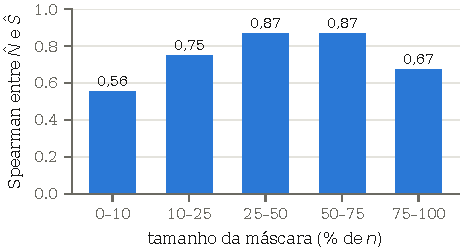
\includegraphics[width=\columnwidth]{correlacao}
\caption{Correlação de Spearman entre $\hat N$ e $\hat S$ entre máscaras de
mesmo tamanho, por faixa de tamanho relativo (média sobre as 99 instâncias).
Valores altos indicam que os dois objetivos ordenam as máscaras da mesma forma.}
\label{fig:correlacao}
\end{figure}

Os dois objetivos, portanto, não são redundantes na região de explicações
pequenas, e mantivemos os três. O conflito tem uma causa visível nas
probabilidades: entre máscaras de até 10 posições, os métodos de busca encontram
alguma com $\widehat{\PN}$ perto de 1, mas a melhor $\widehat{\PS}$ fica perto
de $0{,}55$ (Tabela~\ref{tab:metodos}). Poucos itens bastam para derrubar a
recomendação; poucos itens raramente bastam para sustentá-la contra um
histórico inteiro de itens neutros.

\subsection{Ajuste do NSGA-II}
\label{sec:ajuste}

Nos 30 usuários de ajuste, variamos a população em $\{25,50,100,200\}$ e $M$ em
$\{5,10,20\}$, sempre com $10^5$ passadas e 3 sementes
(Tabela~\ref{tab:ajuste}). Com o orçamento fixo, população e $M$ maiores
significam menos gerações, e o hipervolume cai nas duas direções. Escolhemos
população 25 e $M=10$. Ela é melhor que população 100 com $M=10$ em 27 dos 30
usuários ($p=3\times10^{-6}$ após Holm); a diferença para população 50 com
$M=10$ não é significativa ($p=0{,}23$). O \HVp{} quase não distingue as
configurações (entre $0{,}75$ e $0{,}78$, exceto $0{,}70$ na maior).

\begin{table}[t]
\caption{Ajuste do NSGA-II: hipervolume (todas as máscaras) nos 30 usuários de
ajuste, por tamanho da população e número de fundos $M$.}
\label{tab:ajuste}
\small
\begin{tabular}{@{}lccc@{}}
\toprule
População & $M=5$ & $M=10$ & $M=20$ \\
\midrule
\tabela{ajuste}
\bottomrule
\end{tabular}
\end{table}

\subsection{Comparação entre métodos}

\begin{table*}[t]
\caption{Comparação nas 99 instâncias, com frentes reavaliadas em $M'=100$
fundos independentes. \HVp{}: hipervolume das máscaras com até 10 posições; HV:
de todas as máscaras. Passadas: consultas ao SASRec usadas pela busca. PN e PS:
média da maior $\widehat{\PN}$ e da maior $\widehat{\PS}$ entre máscaras de até
10 posições.}
\label{tab:metodos}
\small
\begin{tabular}{@{}lcccrcc@{}}
\toprule
Método & \HVp & HV & Tamanho da frente & Passadas & PN & PS \\
\midrule
\tabela{metodos}
\bottomrule
\end{tabular}
\end{table*}

A Tabela~\ref{tab:metodos} resume a comparação. O quadro muda conforme a
região da frente.

\paragraph{Explicações pequenas.}
No \HVp{}, o NSGA-II é o melhor método. Ele supera o guloso em 71 das 99
instâncias ($p=1{,}8\times10^{-5}$ após Holm), o ranking por ablação em 89, o
GECE com reinícios em 96 e o AG escalarizado em 97 (todos com
$p<10^{-15}$). A diferença para o AG escalarizado, que usa os mesmos
operadores e o mesmo orçamento, é a mais informativa: dividir o orçamento
entre vetores de pesos cobre pior a região pequena do que uma única população
ordenada por dominância.

\paragraph{Todas as máscaras.}
No HV sem limite de tamanho a ordem se inverte: o guloso é o melhor e supera o
NSGA-II em 81 das 99 instâncias ($p=1{,}1\times10^{-9}$). O ranking por
ablação fica logo atrás usando 4\,615 passadas, menos de 5\% do orçamento. A
razão é estrutural: o guloso e o ranking percorrem todos os tamanhos de $1$ a
$n$, enquanto o NSGA-II, com inicialização esparsa, concentra a busca nas
máscaras pequenas. Como $\hat N$ e $\hat S$ concordam nas máscaras grandes
(Seção~\ref{sec:conflito}), ali uma ordenação simples das posições já basta.

\paragraph{Convergência.}
A Figura~\ref{fig:convergencia} mostra o \HVp{} ao longo da busca. O ranking
por ablação é o mais rápido no início e estaciona; o NSGA-II ultrapassa o
guloso depois de cerca de mil máscaras; o AG escalarizado só se aproxima no
fim, quando já rodou a maior parte dos seus vetores de pesos.

\begin{figure}[t]
\centering
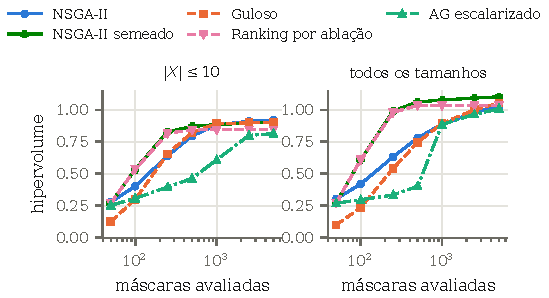
\includegraphics[width=\columnwidth]{convergencia}
\caption{\HVp{} em função do número de máscaras avaliadas (fundos de busca,
média sobre instâncias e sementes). O orçamento completo são 5\,000 máscaras.}
\label{fig:convergencia}
\end{figure}

\paragraph{Recência.}
Os itens escolhidos pelo NSGA-II em máscaras pequenas têm posição relativa
média de $0{,}84$: as explicações se concentram no fim do histórico, como o
GECE já havia observado~\cite{scarcelli2025gece}. Ainda assim, tomar apenas as
$k$ posições mais recentes rende \HVp{} de $0{,}755$, bem abaixo dos métodos
de busca: a recência indica onde procurar, mas não quais itens escolher. O
\HVp{} do NSGA-II varia pouco com a popularidade do alvo ($0{,}91$, $0{,}95$ e
$0{,}90$ nos tercis de baixa, média e alta popularidade).

\subsection{Operadores do NSGA-II}
\label{sec:operadores}

\begin{table}[t]
\caption{Estudo dos operadores do NSGA-II nos 30 usuários de ajuste. Cada
linha muda um único elemento da configuração ajustada.}
\label{tab:operadores}
\small
\begin{tabular}{@{}lccc@{}}
\toprule
Variante & \HVp & HV & Frente \\
\midrule
\tabela{operadores}
\bottomrule
\end{tabular}
\end{table}

A Tabela~\ref{tab:operadores} isola cada escolha. A inicialização esparsa é a
que mais importa: com inicialização uniforme (metade dos bits ligados), o
\HVp{} cai de $0{,}911$ para $0{,}478$, porque a busca gasta o orçamento
descendo de máscaras grandes. Retirar o cruzamento custa cerca de $0{,}10$ de
\HVp{} e quase nada de HV. A taxa de mutação é um compromisso: $0{,}5/n$ ganha
um pouco nas máscaras pequenas (melhor em 23 de 30 usuários, $p=0{,}003$) e
perde no HV geral (pior em 26 de 30); taxas maiores pioram os dois. Mantivemos
$1/n$.

\subsection{Verificação contra a frente exata}
\label{sec:exata}

Nos históricos do experimento, a frente verdadeira é desconhecida. Todo
usuário do MovieLens-20M tem ao menos 19 itens antes do item de teste, de modo
que nenhum histórico real é curto o bastante para ser enumerado. Para medir o
quanto o NSGA-II se aproxima da frente exata, usamos como histórico apenas os
12 itens mais recentes de 20 usuários, com os mesmos candidatos, a mesma regra
de sorteio do alvo e os mesmos fundos. Isso deixa $2^{12}-1=4\,095$ máscaras
por instância, todas avaliadas; a frente exata tem em média 30 máscaras.

\begin{table}[t]
\caption{NSGA-II e busca aleatória contra a frente exata em 20 históricos de
12 itens (5 sementes). HV: fração do hipervolume da frente exata; Frente:
fração das máscaras da frente exata encontradas.}
\label{tab:exata}
\small
\begin{tabular}{@{}rrcccc@{}}
\toprule
 & & \multicolumn{2}{c}{NSGA-II} & \multicolumn{2}{c}{Aleatório} \\
\cmidrule(lr){3-4}\cmidrule(l){5-6}
Máscaras & \% do espaço & HV (\%) & Frente (\%) & HV (\%) & Frente (\%) \\
\midrule
\tabela{exata}
\bottomrule
\end{tabular}
\end{table}

A Tabela~\ref{tab:exata} mostra o resultado. Com 500 máscaras (12\% do
espaço), o NSGA-II atinge $99{,}5\%$ do hipervolume exato e encontra 89\% das
máscaras da frente; com 1\,000, praticamente a frente inteira. A busca
aleatória com as mesmas 1\,000 máscaras encontra 42\% da frente. Em históricos
enumeráveis, portanto, o NSGA-II converge para a frente exata com uma fração
pequena do espaço. Nada garante o mesmo com $n$ até 128, em que o orçamento
cobre uma fração ínfima de $2^n$.

\subsection{AG escalarizado e GECE}

\paragraph{Ajuste do AG escalarizado.}
Para que a comparação não dependa de uma configuração ruim da linha de base,
variamos sua população em $\{10,25,50\}$ e o número de vetores de pesos em
$\{6,10,15\}$ nos usuários de ajuste (Tabela~\ref{tab:escalar}). Nenhuma
configuração vence nos dois critérios: populações pequenas com poucos vetores
têm o maior HV (até $0{,}974$), e as intermediárias o maior \HVp{}. A
configuração usada na comparação principal (população 20, 10 vetores) fica
entre duas que empatam estatisticamente com a melhor em um dos critérios, e a
variação de \HVp{} entre configurações vizinhas é bem menor que a distância
para o NSGA-II na Tabela~\ref{tab:metodos}.

\begin{table}[t]
\caption{Ajuste do AG escalarizado: \HVp{} nos 30 usuários de ajuste, por
população e número de vetores de pesos.}
\label{tab:escalar}
\small
\begin{tabular}{@{}lccc@{}}
\toprule
População & 6 vetores & 10 vetores & 15 vetores \\
\midrule
\tabela{escalar-pequenas}
\bottomrule
\end{tabular}
\end{table}

\paragraph{GECE.}
Como distribuído no TRACE, o GECE sempre encontra um contrafactual válido (495
de 495 execuções) e para depois de 281 consultas em média; com tão poucas
máscaras avaliadas, sua frente fica entre as piores. Com reinícios até o orçamento
completo, ele sobe para perto da linha de base de recência e continua abaixo do
AG escalarizado sobre máscaras. A resposta que o GECE devolve muda uma única
posição em 73\% das execuções. Avaliadas com fundos novos, essas posições têm
$\widehat{\PN}$ média de $0{,}43$, e só 43\% delas são necessárias pelo nosso
critério ($\widehat{\PN}>0{,}5$). Em mais da metade dos casos, portanto, o
contrafactual do GECE depende do item específico que ele inseriu, e não da
posição editada. Isso não é um defeito do GECE, que responde a outra pergunta
(``que edição muda a recomendação?''); mostra que as duas formulações não são
intercambiáveis.

\subsection{Ablações da distribuição de fundo}
\label{sec:ablacao}

Repetimos a busca com dois outros preenchimentos: trechos contíguos do
histórico de outros usuários, mais plausíveis que itens independentes, e
\emph{padding}, em que as posições são simplesmente removidas. Em ambos os
casos as frentes são reavaliadas com os fundos de popularidade da comparação
principal: a pergunta é se explicações encontradas com outro preenchimento
continuam boas (Tabela~\ref{tab:ablacao}).

\begin{table}[t]
\caption{Ablação do preenchimento usado na busca. Todas as frentes são
reavaliadas com fundos de popularidade.}
\label{tab:ablacao}
\small
\begin{tabular}{@{}llcc@{}}
\toprule
Método & Preenchimento na busca & \HVp & HV \\
\midrule
\tabela{ablacao}
\bottomrule
\end{tabular}
\end{table}

Com trechos de outros usuários, os resultados se mantêm: as frentes são tão
boas quanto as da busca original ou ligeiramente melhores, e a ordem dos
métodos na região pequena é a mesma. Com \emph{padding}, todos os métodos
pioram em cerca de 90 das 99 instâncias. Explicações encontradas removendo
itens não se transferem para a substituição: remover desloca a sequência e
muda as posições de todos os itens anteriores, o que é uma intervenção
diferente. As posições escolhidas confirmam a leitura: a similaridade do
cosseno entre as frequências de seleção de cada posição é $0{,}99$ entre
sementes da busca original, $0{,}88$ entre a original e a de outros usuários,
e $0{,}72$ entre a original e a de \emph{padding}.

\subsection{Um exemplo}

\begin{table}[t]
\caption{Uma explicação de quatro itens para a recomendação de \emph{Full
Metal Jacket (1987)} a um usuário com histórico de 40 filmes
($\widehat{\PN}=0{,}97$, $\widehat{\PS}=0{,}86$). A posição 40 é a mais
recente.}
\label{tab:exemplo}
\small
\begin{tabular}{@{}rl@{}}
\toprule
Posição & Filme \\
\midrule
\tabela{exemplo}
\bottomrule
\end{tabular}
\end{table}

\begin{figure}[t]
\centering
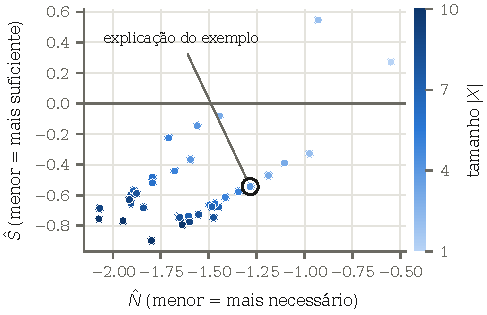
\includegraphics[width=\columnwidth]{exemplo-frente}
\caption{Frente do NSGA-II para a instância da Tabela~\ref{tab:exemplo}
(máscaras de até 10 posições, uma semente). O círculo marca a explicação da
tabela.}
\label{fig:exemplo}
\end{figure}

A Tabela~\ref{tab:exemplo} mostra uma explicação da frente do NSGA-II.
Substituir esses quatro filmes tira \emph{Full Metal Jacket} do top-10 em 97\%
dos fundos, e mantê-los sozinhos o sustenta em 86\%. A melhor explicação de um
único item (o filme mais recente, \emph{Reservoir Dogs}) é necessária em 75\%
dos fundos, mas suficiente em apenas 40\%. A Figura~\ref{fig:exemplo} mostra o
que uma resposta única esconderia: o usuário da explicação pode trocar tamanho
por força, e as máscaras maiores avançam nos dois objetivos ao mesmo tempo.

%% ---- 7. Discussão e Conclusão -----------------------------------------------
\section{Discussão e Conclusão}

Formulamos a explicação contrafactual de uma recomendação sequencial como a
busca de conjuntos de posições do histórico sob três objetivos (necessidade,
suficiência e tamanho), estimados por intervenções com fundos fixos, e a
resolvemos com algoritmos evolutivos multiobjetivo sobre máscaras binárias. A
proposta previa que uma busca multiobjetivo cobriria uma frente melhor que o
mesmo orçamento gasto em buscas escalarizadas, e apontava como risco que $N$ e
$S$ fossem quase redundantes. As duas coisas ocorreram, em regiões diferentes.
Nas explicações pequenas, $N$ e $S$ concordam só moderadamente, os algoritmos
baseados em dominância de Pareto são os melhores métodos, contra a busca
escalarizada, o guloso, o Shapley e o GECE, e manter $S$ como objetivo não
custa, em média, nada em necessidade e tamanho. Nas máscaras grandes, $N$ e
$S$ quase coincidem, e métodos que percorrem todos os tamanhos vencem o NSGA-II
original no MovieLens; só a variante semeada, posterior à comparação
planejada, vence ali. As conclusões dos métodos centrais se repetem em
instâncias novas e no Zvuk.

\paragraph{Limitações.}
(i)~Não há avaliação com usuários: mostramos que as frentes contêm explicações
pequenas, necessárias e às vezes suficientes, não que uma frente seja mais útil
a quem a lê do que uma resposta única. (ii)~Vários experimentos foram decididos
depois da comparação planejada ($\dagger$); a confirmação em dados novos cobre
os métodos centrais, mas não o NSGA-III, o Shapley e a variante só $(N,C)$, de
que depende o terceiro resultado. (iii)~A distribuição de fundo define o que
``suficiente'' significa, e trocá-la muda as explicações
(Apêndice~\ref{sec:ablacao}). (iv)~O ajuste foi desigual (12 configurações
para o NSGA-II, menos para os demais) e o MOEA/D só foi testado com pesos
uniformes; como os três algoritmos baseados em dominância diferem por menos de
$0{,}01$ de \HVp{}, mais ajuste poderia mudar a ordem entre eles. Outras
limitações estão no Apêndice~\ref{ap:limitacoes}.

\paragraph{Trabalho futuro.}
Uma semeadura que não custe nada nas explicações pequenas (por exemplo, só
com máscaras pequenas), operadores que usem a estrutura do problema (mutação
enviesada para os itens recentes), outras arquiteturas de recomendador e uma
avaliação com usuários.

\paragraph{Reprodutibilidade.}
O código, os arquivos de resultados usados nas tabelas e figuras, os roteiros
que as geram e os comandos de cada execução estão no repositório do projeto
(\url{https://github.com/jorgesilva2407/moo-seqrec-explanations}).


\bibliographystyle{ACM-Reference-Format}
\bibliography{referencias}

\end{document}
